\documentclass[tikz,border=4pt]{standalone}
\usepackage[T1]{fontenc}
\usepackage[utf8]{inputenc}
\usepackage{helvet}
\renewcommand{\familydefault}{\sfdefault}
\definecolor{treffer}{HTML}{E69F00}
\definecolor{niete}{HTML}{0072B2}
\tikzset{
  los/.style={draw=black!70, fill=white, rounded corners=3pt, minimum width=2.2cm, minimum height=1.5cm, line width=0.8pt, font=\Large\bfseries},
  ergebnis/.style={circle, draw=black!60, minimum size=0.85cm, inner sep=0pt, font=\bfseries\color{white}},
}
\begin{document}
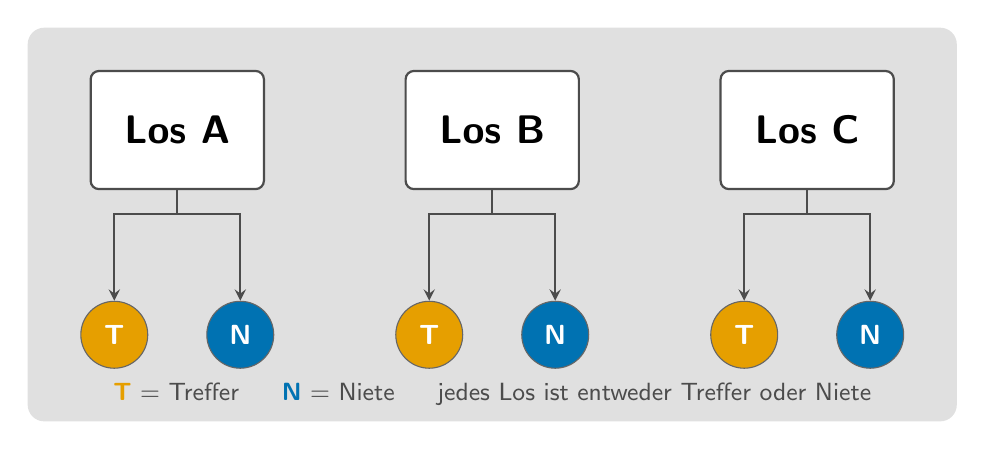
\begin{tikzpicture}
  \fill[black!12, rounded corners=6pt] (-1.9,-3.7) rectangle (9.9,1.3);
  \foreach \x/\l in {0/A, 4/B, 8/C} {
    \node[los] (\l) at (\x,0) {Los \l};
    \node[ergebnis, fill=treffer] (T\l) at (\x-0.8,-2.6) {T};
    \node[ergebnis, fill=niete]   (N\l) at (\x+0.8,-2.6) {N};
    \draw[-stealth, line width=0.8pt, black!70] (\l.south) -- ++(0,-0.3) -| (T\l.north);
    \draw[-stealth, line width=0.8pt, black!70] (\l.south) -- ++(0,-0.3) -| (N\l.north);
  }
  \node[font=\small, text=black!70] at (4,-3.35) {\textcolor{treffer}{\textbf{T}} = Treffer \quad\ \textcolor{niete}{\textbf{N}} = Niete \quad\ jedes Los ist entweder Treffer oder Niete};
\end{tikzpicture}
\end{document}
